\documentclass[10pt]{beamer}
\usetheme[
%%% option passed to the outer theme
%    progressstyle=fixedCircCnt,   % fixedCircCnt, movingCircCnt (moving is deault)
  ]{Feather}
  
% If you want to change the colors of the various elements in the theme, edit and uncomment the following lines

% Change the bar colors:
\setbeamercolor{Feather}{fg=black!20,bg=black}

% Change the color of the structural elements:
\setbeamercolor{structure}{fg=black}

% Change the frame title text color:
%\setbeamercolor{frametitle}{fg=blue}

% Change the normal text color background:
%\setbeamercolor{normal text}{fg=black,bg=gray!10}

%-------------------------------------------------------
% INCLUDE PACKAGES
%-------------------------------------------------------

\usepackage[utf8]{inputenc}
\usepackage[polish]{babel}
\usepackage{polski}
\usepackage[T1]{fontenc}
\usepackage{helvet}
\usepackage{booktabs}
\usepackage{array}
\usepackage{setspace}
\usepackage{graphicx}
\usepackage{caption}
\usepackage{soul}


%-------------------------------------------------------
% DEFFINING AND REDEFINING COMMANDS
%-------------------------------------------------------
\DeclareCaptionLabelSeparator{kropka}{. }
\setbeamertemplate{caption}[numbered]
\captionsetup[figure]{labelformat=simple, labelsep=kropka}
\captionsetup[table]{labelformat=simple, labelsep=kropka}
\addto\captionspolish{\renewcommand{\tablename}{Tabela}}

\newcolumntype{k}[1]{>{\centering\arraybackslash}m{#1}}

% colored hyperlinks
\newcommand{\chref}[2]{
  \href{#1}{{\usebeamercolor[bg]{Feather}#2}}
}

%-------------------------------------------------------
% INFORMATION IN THE TITLE PAGE
%-------------------------------------------------------

\title[Polska szkoła sztucznej inteligencji – zbiory przybliżone] % [] is optional - is placed on the bottom of the sidebar on every slide
{ % is placed on the title page
      \textbf{Zbiory przybliżone}
}

\subtitle[]
{
      \textbf{Polska szkoła sztucznej inteligencji}
}

\author[Jan Gromko]
{
\textbf{Jan Gromko}
}

\institute[SKN Math4You WI PB]
{
      Studenckie Koło Naukowe Math4You\\
      Wydział Informatyki Politechniki Białostockiej
}

\date{22 kwietnia 2017 r.}


\begin{document}


{\1% wybór pliku na tło
\begin{frame}[plain,noframenumbering]
  \titlepage
\end{frame}}


\begin{frame}{Plan referatu}{}
\tableofcontents
\end{frame}

%-------------------------------------------------------
\section{Wprowadzenie}
%-------------------------------------------------------
\subsection{Czym są zbiory przybliżone – historia i idea}
\begin{frame}{Historia i idea}
\begin{spacing}{1.5}
\begin{itemize}
\item Teoria zaproponowana w 1982 r. przez prof. Zdzisława Pawlaka.
\item Wprowadzona jako nowe matematyczne podejście do pojęć nieostrych i metoda analizy danych.
\end{itemize}
\end{spacing}

\end{frame}

%-------------------------------------------------------
\subsection{Podstawowe pojęcia}
\begin{frame}{Podstawy}
\begin{spacing}{1.5}
\begin{itemize}
\item Zbiory przybliżone oparte są o logikę trójwartościową;
\item zbiór przybliżony jest zbiorem niedefiniowalnym -- nie można go jednoznacznie scharakteryzować na podstawie własności jego elementów.
\end{itemize}

\end{spacing}
\end{frame}


\begin{frame}{Przykład}
\begin{center}
\begin{table}
\begin{tabular}{|k{1.2cm}|k{1.8cm}|k{1.8cm}|k{2.2cm}|k{1.4cm}|@{}m{0pt}@{}}
\hline
\textit{Pacjent} & \textit{Ból głowy} & \textit{Ból mięśni} & \textit{Temperatura} &  \textit{Grypa} &\\[1ex]
\hline
1 & nie & tak & podwyższona & tak &\\[1ex]
2 & tak & nie & podwyższona & tak &\\[1ex]
3 & tak & tak & wysoka & tak &\\[1ex]
4 & nie & tak & normalna & nie &\\[1ex]
5 & tak & nie & podwyższona & nie &\\[1ex]
6 & nie & nie & wysoka & tak &\\[1ex]
\hline
\end{tabular}
\caption{Tablica decyzyjna przykładowego zbioru.}
\end{table}
\end{center}
\end{frame}




\begin{frame}
\frametitle{Podstawowe pojęcia}
\begin{spacing}{1.7}
\begin{flushleft}
$S = (U, A, V, f)$ -- system informacyjny\\
$U$ -- zbiór obiektów (\textit{uniwersum})\\
$A$ -- zbiór atrybutów\\
$V = \bigcup\limits_{a \in A} V_{a}$ -- zbiór wszystkich możliwych wartości atrybutów\\
$V_{a}$ -- dziedzina atrybutu $a \in A$\\
$f : U \times A \rightarrow V$ -- funkcja informacyjna\\
\end{flushleft}
\end{spacing}
\end{frame}


\begin{frame}
\frametitle{Podstawowe pojęcia}
\begin{spacing}{1.7}
\begin{flushleft}
$DT = (U, C, D, V, f)$ -- tablica decyzyjna\\
$C$ -- zbiór atrybutów warunkowych\\
$D$ -- zbiór atrybutów decyzyjnych\\
$A = C \cup D$ -- zbiór atrybutów\\
\end{flushleft}
\end{spacing}
\end{frame}


\begin{frame}
\frametitle{Podstawowe pojęcia}
\begin{table}
\begin{tabular}{|k{1.2cm}|k{1.8cm}|k{1.8cm}|k{2.2cm}|k{1.4cm}|@{}m{0pt}@{}}
\hline
\textit{Pacjent} & \textit{Ból głowy} & \textit{Ból mięśni} & \textit{Temperatura} &  \textit{Grypa} &\\[1ex]
\hline
1 & nie & tak & podwyższona & tak &\\[1ex]
2 & tak & nie & podwyższona & tak &\\[1ex]
3 & tak & tak & wysoka & tak &\\[1ex]
4 & nie & tak & normalna & nie &\\[1ex]
5 & tak & nie & podwyższona & nie &\\[1ex]
6 & nie & nie & wysoka & tak &\\[1ex]
\hline
\end{tabular}
\caption{Tablica decyzyjna przykładowego zbioru.}
\end{table}
\begin{spacing}{1}
\begin{flushleft}
$U$ -- pacjenci\\
$C = \lbrace$\textit{ból głowy, ból mięśni, temperatura}$\rbrace$, $D$ -- \textit{grypa}\\
\end{flushleft}
\end{spacing}
\end{frame}





\begin{frame}{Reguły decyzyjne}
\begin{spacing}{1.5}
\textbf{Problem:}\\
Znaleźć zależność między występowaniem/niewystępowaniem grypy a symptomami występującymi u pacjentów, czyli znaleźć zależność między atrybutem decyzyjnym a wartościami atrybutów warunkowych, opisujących poszczególne obiekty.
\end{spacing}
\end{frame}


\begin{frame}{Sprzeczności w zbiorze}
\renewcommand{\arraystretch}{1}
\begin{center}
\begin{table}
\begin{tabular}{|k{1.2cm}|k{1.8cm}|k{1.8cm}|k{2.2cm}|k{1.4cm}|@{}m{0pt}@{}}
\hline
\textit{Pacjent} & \textit{Ból głowy} & \textit{Ból mięśni} & \textit{Temperatura} &  \textit{Grypa} &\\[1ex]
\hline
2 & tak & nie & podwyższona & tak &\\[1ex]
5 & tak & nie & podwyższona & nie &\\[1ex]
\hline
\end{tabular}
\caption{Sprzeczne informacje w zbiorze -- przypadki, których nie można jednoznacznie sklasyfikować.}
\end{table}
\end{center}
\end{frame}


\begin{frame}{Podstawowe pojęcia}
\begin{block}{Relacja nierozróżnialności}
Relację nierozróżnialności zdefiniowana jest jako
$$IND(B)=\lbrace (x,y) \in U \times U: \forall_{a \in B}~~a(x)=a(y) \rbrace,$$
gdzie $B \subseteq A$.\\
$\newline$
Jeśli $(x, y) \in IND(B)$, wówczas obiekty $x$ i $y$ są nierozróżnialne ze~względu na podzbiór atrybutów $B$.
\end{block}
\end{frame}


\begin{frame}{Przykład -- analiza danych}
\begin{spacing}{1.5}
\textbf{W oparciu o posiadane dane, można stwierdzić, że:}\\
\begin{itemize}
\item $\lbrace 1,3,6 \rbrace$ to zbiór przypadków, które (na podstawie atrybutów warunkowych) możemy \textit{jednoznacznie} zaklasyfikować do grupy pacjentów chorych na grypę;
\item $\lbrace 1,2,3,5,6 \rbrace$ to zbiór przypadków, które \textit{mogą} być zakwalifikowanie jako pacjenci chorzy na grypę;
\item $\lbrace 2,5 \rbrace$ to zbiór przypadków, które nie mogą być jednoznacznie zaklasyfikowane jako pacjenci, którzy są lub nie są chorzy na~grypę.
\end{itemize}
\end{spacing}
\end{frame}


\begin{frame}{Podstawowe pojęcia}
\begin{spacing}{1.2}
\begin{block}{Dolne przybliżenie}
Wszystkie te elementy, które można jednoznacznie zaklasyfikować do danego zbioru, według posiadanej wiedzy na ich temat.
\end{block}
\begin{block}{Górne przybliżenie}
Wszystkie te elementy, których przynależności do danego zbioru nie można wykluczyć.
\end{block}
\end{spacing}
\end{frame}


\begin{frame}{Podstawowe pojęcia}
\begin{center}
\begin{figure}
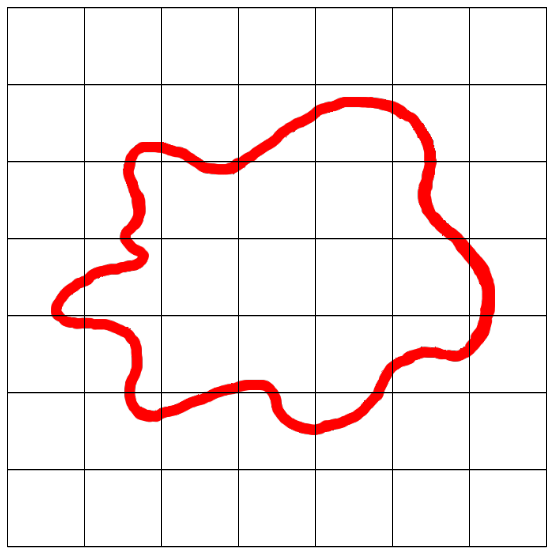
\includegraphics[width=0.55\textwidth]{Grafiki/plama.png}
\caption{Przykładowy zbiór.}
\end{figure}
\end{center}
\end{frame}


\begin{frame}{Dolne przybliżenie}
\begin{center}
\begin{figure}
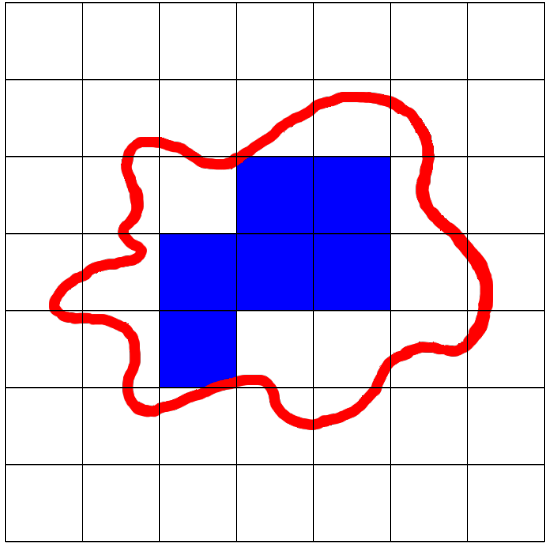
\includegraphics[width=0.55\textwidth]{Grafiki/dolne_przyblizenie.png}
\caption{Dolne przybliżenie zbioru.}
\end{figure}

\end{center}
\end{frame}


\begin{frame}{Górne przybliżenie}
\begin{center}
\begin{figure}
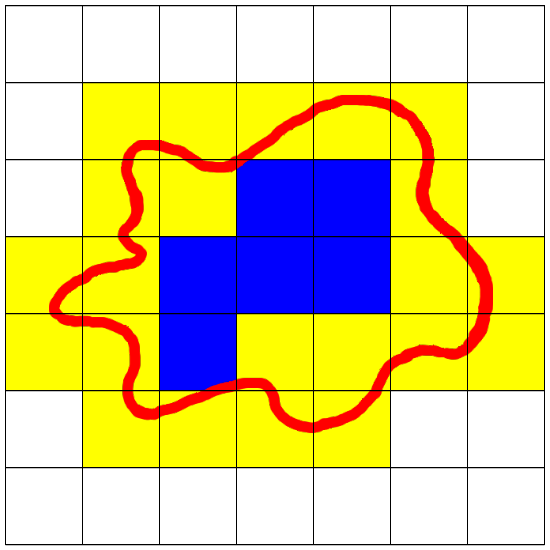
\includegraphics[width=0.55\textwidth]{Grafiki/gorne_przyblizenie.png}
\caption{Górne przybliżenie zbioru.}
\end{figure}
\end{center}
\end{frame}


\begin{frame}{Obszar brzegowy}
\begin{center}
\begin{figure}
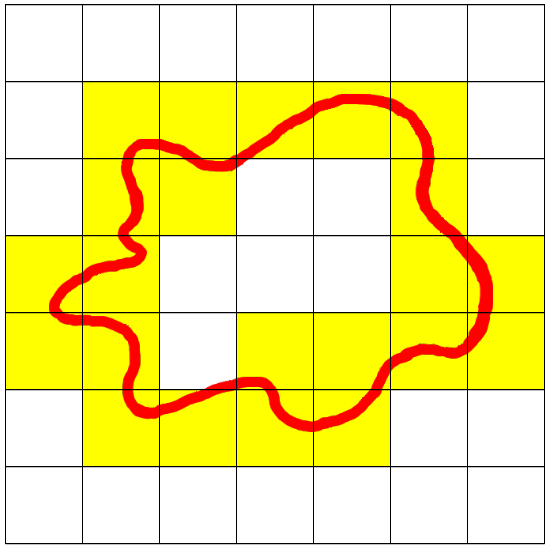
\includegraphics[width=0.55\textwidth]{Grafiki/obszar_brzegowy.png}
\caption{Obszar brzegowy zbioru.}
\end{figure}

\end{center}
\end{frame}



\begin{frame}{Podstawy}
\begin{spacing}{1.5}
\begin{itemize}
\item Zbiory przybliżone oparte są o logikę trójwartościową;
\item zbiór przybliżony jest zbiorem niedefiniowalnym -- nie można go jednoznacznie scharakteryzować na podstawie własności jego~elementów;
\item \textbf{zbiór przybliżony można jednak scharakteryzować za~pomocą dwóch zbiorów definiowalnych -- dolnego i~górnego przybliżenia.}
\end{itemize}

\end{spacing}
\end{frame}


\section{Problem redukcji}


\begin{frame}
\begin{Huge}
\textbf{Problem redukcji}
\end{Huge}
\end{frame}

\subsection{Istota problemu redukcji}
\begin{frame}{Istota problemu}
\begin{spacing}{1.5}
\textbf{Czy można zredukować zbiór pod~względem atrybutów w~ten~sposób, by~zachowana była rozróżnialność elementów z~oryginalnego zbioru?}
\end{spacing}
\end{frame}

\begin{frame}
\frametitle{Redukcja}
\begin{spacing}{1.5}
\begin{block}{Zbiór niezależny}
Zbiór atrybutów $B_{1} \subset A$ jest \textit{niezależny} w danym systemie informacyjnym, jeśli dla każdego $B_{2} \subset B_{1}$ zachodzi $IND(B_{1}) \neq IND(B_{2})$.
\end{block}

\begin{block}{Redukt}
\textit{Reduktem} zbioru atrybutów $B_{1} \subseteq A$ nazywamy każdy niezależny zbiór $B_{2} \subseteq B_{1}$, dla którego $IND(B_{1}) = IND(B_{2})$, przy czym $B_{2}$ powinien być 
jak najmniej liczny. Może istnieć wiele reduktów.
\end{block}
\end{spacing}
\end{frame}


\begin{frame}{Tworzenie macierzy rozróżnialności}{Zasady}
\begin{spacing}{1.5}
\begin{itemize}
\item W każdej komórce macierzy rozróżnialności umieszczane są atrybuty rozróżniające każde dwa obiekty,
\item rozróżniamy jedynie obiekty należące do różnych klas decyzyjnych,
\item wystarczające jest wypełnienie jedynie połowy macierzy (dzielonej według głównej przekątnej), ponieważ jeśli obiekt $x_{1}$ jest rozróżnialny od atrybutu $x_{2}$ przez zbiór atrybutów $K$, to obiekt $x_{2}$ jest rozróżnialny od atrybutu $x_{1}$ przez ten sam zbiór atrybutów.
\end{itemize}
\end{spacing}
\end{frame}


\begin{frame}{Macierz rozróżnialności}
\renewcommand{\arraystretch}{1}
\begin{center}
\begin{table}
\begin{tabular}{|k{1cm}|k{1cm}|k{1cm}|k{1cm}|k{1cm}|k{1cm}|k{1cm}|@{}m{0pt}@{}}
\hline
& 1 & 2 & 3 & 4 & 5 & 6&\\[1ex]
\hline
1 & $\emptyset$ & -- & -- & -- & -- & -- &\\[1ex]
\hline
2 & $\emptyset$ & $\emptyset$ & -- & -- & -- & -- &\\[1ex]
\hline
3 & $\emptyset$ & $\emptyset$ & $\emptyset$ & -- & -- & -- &\\[1ex]
\hline
4 & t & g, m, t & g, t & $\emptyset$ & -- & -- &\\[1ex]
\hline
5 & g, m & $\emptyset$ & m, t & $\emptyset$ & $\emptyset$ & -- &\\[1ex]
\hline
6 &$\emptyset$ & $\emptyset$ & $\emptyset$ & m, t & g, t & $\emptyset$ &\\[1ex]
\hline
\end{tabular}
\caption{Macierz rozróżnialności.}
\end{table}

\end{center}

\begin{flushleft}
\textit{g} -- ból głowy; 
\textit{m} -- ból mięśni; 
\textit{t} -- temperatura
\end{flushleft}

\end{frame}


\begin{frame}{Tworzenie macierzy rozróżnialności}
\renewcommand{\arraystretch}{1}
\begin{center}

\begin{table}
\begin{tabular}{|k{1.2cm}|k{1.8cm}|k{1.8cm}|k{2.2cm}|k{1.4cm}|@{}m{0pt}@{}}
\hline
\textit{Pacjent} & \textit{Ból głowy} & \textit{Ból mięśni} & \textit{Temperatura} &  \textit{Grypa} &\\[1ex]
\hline
1 & nie & tak & podwyższona & tak &\\[1ex]
5 & tak & nie & podwyższona & nie &\\[1ex]
\hline
\end{tabular}
\caption{Fragment tablicy decyzyjnej.}
\end{table}

\begin{table}
\begin{tabular}{|k{1cm}|k{1cm}|k{1cm}|k{1cm}|k{1cm}|k{1cm}|k{1cm}|@{}m{0pt}@{}}
\hline
& 1 & 2 & 3 & 4 & 5 & 6 & \\[1ex]
\hline
5 & \alert{g, m} & ? & ? & $\emptyset$ & $\emptyset$ & -- &\\[1ex]
\hline
\end{tabular}
\caption{Fragment macierzy rozróżnialności.}
\end{table}

\end{center}

\end{frame}


\begin{frame}{Tworzenie macierzy rozróżnialności}
\renewcommand{\arraystretch}{1}
\begin{center}

\begin{table}
\begin{tabular}{|k{1.2cm}|k{1.8cm}|k{1.8cm}|k{2.2cm}|k{1.4cm}|@{}m{0pt}@{}}
\hline
\textit{Pacjent} & \textit{Ból głowy} & \textit{Ból mięśni} & \textit{Temperatura} &  \textit{Grypa} &\\[1ex]
\hline
2 & tak & nie & podwyższona & tak &\\[1ex]
5 & tak & nie & podwyższona & nie &\\[1ex]
\hline
\end{tabular}
\caption{Fragment tablicy decyzyjnej.}
\end{table}

\begin{table}
\begin{tabular}{|k{1cm}|k{1cm}|k{1cm}|k{1cm}|k{1cm}|k{1cm}|k{1cm}|@{}m{0pt}@{}}
\hline
& 1 & 2 & 3 & 4 & 5 & 6 & \\[1ex]
\hline
5 & g, m & \alert{$\emptyset$} & ? & $\emptyset$ & $\emptyset$ & -- &\\[1ex]
\hline
\end{tabular}
\caption{Fragment macierzy rozróżnialności.}
\end{table}

\end{center}

\end{frame}


\begin{frame}{Tworzenie macierzy rozróżnialności}
\renewcommand{\arraystretch}{1}
\begin{center}

\begin{table}
\begin{tabular}{|k{1.2cm}|k{1.8cm}|k{1.8cm}|k{2.2cm}|k{1.4cm}|@{}m{0pt}@{}}
\hline
\textit{Pacjent} & \textit{Ból głowy} & \textit{Ból mięśni} & \textit{Temperatura} &  \textit{Grypa} &\\[1ex]
\hline
3 & tak & tak & wysoka & tak &\\[1ex]
5 & tak & nie & podwyższona & nie &\\[1ex]
\hline
\end{tabular}
\caption{Fragment tablicy decyzyjnej.}
\end{table}

\begin{table}
\begin{tabular}{|k{1cm}|k{1cm}|k{1cm}|k{1cm}|k{1cm}|k{1cm}|k{1cm}|@{}m{0pt}@{}}
\hline
& 1 & 2 & 3 & 4 & 5 & 6 & \\[1ex]
\hline
5 & g, m & $\emptyset$ & \alert{m, t} & $\emptyset$ & $\emptyset$ & -- &\\[1ex]
\hline
\end{tabular}
\caption{Fragment macierzy rozróżnialności.}
\end{table}

\end{center}

\end{frame}


\begin{frame}{Macierz rozróżnialności -- oryginalny zbiór}
\renewcommand{\arraystretch}{1}
\begin{center}
\begin{table}
\begin{tabular}{|k{1cm}|k{1cm}|k{1cm}|k{1cm}|k{1cm}|k{1cm}|k{1cm}|@{}m{0pt}@{}}
\hline
& 1 & 2 & 3 & 4 & 5 & 6&\\[1ex]
\hline
1 & $\emptyset$ & -- & -- & -- & -- & -- &\\[1ex]
\hline
2 & $\emptyset$ & $\emptyset$ & -- & -- & -- & -- &\\[1ex]
\hline
3 & $\emptyset$ & $\emptyset$ & $\emptyset$ & -- & -- & -- &\\[1ex]
\hline
4 & t & g, m, t & g, t & $\emptyset$ & -- & -- &\\[1ex]
\hline
5 & g, m & $\emptyset$ & m, t & $\emptyset$ & $\emptyset$ & -- &\\[1ex]
\hline
6 &$\emptyset$ & $\emptyset$ & $\emptyset$ & m, t & g, t & $\emptyset$ &\\[1ex]
\hline
\end{tabular}
\caption{Macierz rozróżnialności.}
\end{table}

\end{center}

\end{frame}



\begin{frame}{Macierz rozróżnialności -- redukcja}
\renewcommand{\arraystretch}{1}
\begin{center}
\begin{table}
\begin{tabular}{|k{1cm}|k{1cm}|k{1cm}|k{1cm}|k{1cm}|k{1cm}|k{1cm}|@{}m{0pt}@{}}
\hline
& 1 & 2 & 3 & 4 & 5 & 6 &\\[1ex]
\hline
1 & $\emptyset$ & -- & -- & -- & -- & --&\\[1ex]
\hline
2 & $\emptyset$ & $\emptyset$ & -- & -- & -- & --&\\[1ex]
\hline
3 & $\emptyset$ & $\emptyset$ & $\emptyset$ & -- & -- & --&\\[1ex]
\hline
4 & t & g, t & g, t & $\emptyset$ & -- & --&\\[1ex]
\hline
5 & g & $\emptyset$ & t & $\emptyset$ & $\emptyset$ & --&\\[1ex]
\hline
6 &$\emptyset$ & $\emptyset$ & $\emptyset$ & t & g, t & $\emptyset$&\\[1ex]
\hline
\end{tabular}
\caption{Macierz rozróżnialności po redukcji.}
\end{table}

\end{center}

\end{frame}


\subsection{Prosty algorytm wyznaczania reduktu}

\begin{frame}{Prosty algorytm wyznaczania reduktu}
\begin{spacing}{1.5}
\begin{enumerate}
\item Zliczenie wystąpień atrybutów w macierzy rozróżnialności.
\item Wybór atrybutu występującego najliczniej w macierzy rozróżnialności; dodanie wybranego atrybutu do wynikowego zbioru atrybutów $Red$.
\item Wykreślenie komórek zawierających wybrany atrybut.
\item Jeśli wszystkie komórki zostały wykreślone, wynikiem jest uzyskany zbiór $Red$, w przeciwnym razie powrót do kroku 1.
\end{enumerate}
\end{spacing}
\end{frame}



\begin{frame}{Prosty algorytm redukcji}
\renewcommand{\arraystretch}{1}
\begin{center}
\begin{table}
\begin{tabular}{|k{1cm}|k{1cm}|k{1cm}|k{1cm}|k{1cm}|k{1cm}|k{1cm}|@{}m{0pt}@{}}
\hline
& 1 & 2 & 3 & 4 & 5 & 6&\\[1ex]
\hline
4 & t & g, m, t & g, t & $\emptyset$ & -- & -- &\\[1ex]
\hline
5 & g, m & $\emptyset$ & m, t & $\emptyset$ & $\emptyset$ & -- &\\[1ex]
\hline
6 &$\emptyset$ & $\emptyset$ & $\emptyset$ & m, t & g, t & $\emptyset$ &\\[1ex]
\hline
\end{tabular}
\caption{Fragment macierzy rozróżnialności zawierający istotne dane.}
\end{table}
$\newline$
\begin{spacing}{1.5}
g -- 4~~~~~~~~~~~~~m -- 4~~~~~~~~~~~~~\alert{t -- 6}\\
\end{spacing}
\end{center}
\end{frame}


\begin{frame}{Prosty algorytm redukcji}
\renewcommand{\arraystretch}{1}
\begin{center}
\begin{table}
\begin{tabular}{|k{1cm}|k{1cm}|k{1cm}|k{1cm}|k{1cm}|k{1cm}|k{1cm}|@{}m{0pt}@{}}
\hline
& 1 & 2 & 3 & 4 & 5 & 6&\\[1ex]
\hline
4 & \st{t} & \st{g, m, t} & \st{g, t} & $\emptyset$ & -- & -- &\\[1ex]
\hline
5 & g, m & $\emptyset$ & \st{m, t} & $\emptyset$ & $\emptyset$ & -- &\\[1ex]
\hline
6 &$\emptyset$ & $\emptyset$ & $\emptyset$ & \st{m, t} & \st{g, t} & $\emptyset$ &\\[1ex]
\hline
\end{tabular}
\caption{Fragment macierzy rozróżnialności zawierający istotne dane.}
\end{table}
$\newline$
\begin{spacing}{1.5}
$Red = \lbrace t \rbrace$\\
\alert{g -- 1~~~~~~~~~~~~~m -- 1}
\end{spacing}
\end{center}
\end{frame}


\begin{frame}{Prosty algorytm redukcji}
\renewcommand{\arraystretch}{1}
\begin{center}
\begin{table}
\begin{tabular}{|k{1cm}|k{1cm}|k{1cm}|k{1cm}|k{1cm}|k{1cm}|k{1cm}|@{}m{0pt}@{}}
\hline
& 1 & 2 & 3 & 4 & 5 & 6&\\[1ex]
\hline
4 & \st{t} & \st{g, m, t} & \st{g, t} & $\emptyset$ & -- & -- &\\[1ex]
\hline
5 & \st{g, m} & $\emptyset$ & \st{m, t} & $\emptyset$ & $\emptyset$ & -- &\\[1ex]
\hline
6 &$\emptyset$ & $\emptyset$ & $\emptyset$ & \st{m, t} & \st{g, t} & $\emptyset$ &\\[1ex]
\hline
\end{tabular}
\caption{Fragment macierzy rozróżnialności zawierający istotne dane.}
\end{table}
$\newline$
\begin{spacing}{1.5}
$Red = \lbrace t, g \rbrace \vee Red = \lbrace t, m \rbrace$\\
\end{spacing}
\end{center}
\end{frame}


\begin{frame}{Rdzeń}
\renewcommand{\arraystretch}{1}
\begin{center}
\begin{table}
\begin{tabular}{|k{1cm}|k{1cm}|k{1cm}|k{1cm}|k{1cm}|k{1cm}|k{1cm}|@{}m{0pt}@{}}
\hline
& 1 & 2 & 3 & 4 & 5 & 6&\\[1ex]
\hline
1 & $\emptyset$ & -- & -- & -- & -- & -- &\\[1ex]
\hline
2 & $\emptyset$ & $\emptyset$ & -- & -- & -- & -- &\\[1ex]
\hline
3 & $\emptyset$ & $\emptyset$ & $\emptyset$ & -- & -- & -- &\\[1ex]
\hline
4 & \alert{t} & g, m, t & g, t & $\emptyset$ & -- & -- &\\[1ex]
\hline
5 & g, m & $\emptyset$ & m, t & $\emptyset$ & $\emptyset$ & -- &\\[1ex]
\hline
6 &$\emptyset$ & $\emptyset$ & $\emptyset$ & m, t & g, t & $\emptyset$ &\\[1ex]
\hline
\end{tabular}
\caption{Macierz rozróżnialności oryginalnego zbioru.}
\end{table}
\begin{spacing}{1.5}
$Red = \lbrace \alert{t}, g \rbrace \vee Red = \lbrace \alert{t}, m \rbrace$\\
\end{spacing}
\end{center}
\end{frame}


\subsection{Alternatywne metody wyznaczania reduktu}

\begin{frame}{Problem złożoności wyznaczania reduktu}
\begin{spacing}{1.5}
Wyznaczanie reduktu w zbiorze przybliżonym jest problemem NP-zupełnym -- nie jest możliwe znalezienie rozwiązania w~czasie~wielomianowym.
\end{spacing}
\end{frame}


\begin{frame}{Alternatywne metody wyznaczania reduktu}
\begin{spacing}{1.5}
Rozwiązania sprzętowe:\\
\begin{itemize}
\item specjalizowane układy programowalne.
\end{itemize}

Rozwiązania przybliżone -- wykorzystanie innych metod sztucznej~inteligencji:\\
\begin{itemize}
\item algorytmy ewolucyjne,
\item algorytmy mrówkowe,
\item inteligencja roju,
\item metody połączone.
\end{itemize}
\end{spacing}
\end{frame}


\begin{frame}{Rozwiązania sprzętowe}
\begin{spacing}{1.2}
\begin{itemize}
\item Opis zbiorów przybliżonych z wykorzystaniem sieci komórkowych (\textit{cellular networks}; na tej podstawie w 1994 r. opracowana została koncepcja PRSComp (\textit{Parallel Rough Sets COMPuter}) --\\Rybiński, Muraszkiewicz (1984);
\item idea samouczącego się systemu, wykorzystującego sieci komórkowe -- uczenie systemu w warstwie oprogramowania, na~podstawie wyników tworzona jest warstwa sprzętowa --\\Lewis, Perkowski, Jóźwiak (1999);
\item implementacja systemu opartego o sieci komórkowe -- Dharmadhikari, Ngo, Lewisa (1999);
\item koncepcja RSP (\textit{Roug Set Processor}) -- Pawlak (2004);
\end{itemize}
\end{spacing}
\end{frame}


\begin{frame}{Rozwiązania sprzętowe (cd.)}
\begin{spacing}{1.2}
\begin{itemize}
\item idea systemu wspierającego w sposób sprzętowy minimalizację funkcji logicznych, tworzonych na podstawie macierzy rozróżnialności -- Kanasugi, Yokoyama (2001);
\item implementacja wyżej wymienionego rozwiązania w FPGA, 700-krotne skrócenie czasu obliczeń w porównaniu do tradycyjnych rozwiązań -- Kanasugi, Matsumoto (2007);
\item koprocesor wspomagający sprzętowo niektóre operacje na ZP -- Tiwari, Kothari (2015);
\item implementacje sprzętowe na FPGA i~CPLD metod ZP od~operacji podstawowych (jak np. obliczanie aproksymacji), przez wyznaczanie rdzeni i~reduktów, po~generowanie reguł decyzyjnych~-- Kopczyński (2016).
\end{itemize}
\end{spacing}
\end{frame}



\begin{frame}{Rozwiązania przybliżone}
\begin{spacing}{1.2}
\begin{itemize}
\item Algorytmy genetyczne, oparte o sprowadzenie problemu redukcji do~problemu pokrycia kolumnowego macierzy, w~której kolumny odpowiadają atrybutom, a~wiersze parom obiektów, które~wymagają rozróżnienia -- Wróblewski (2001);
\item redukcja ZP przy pomocy algorytmów mrówkowych --\\Jensen, Shen (2003);
\item algorytm hybrydowy, łączący algorytmy mrówkowe i inteligencję roju -- Pratiwi, Choo, Muda (2011);
\end{itemize}
\end{spacing}
\end{frame}


\begin{frame}{Rozwiązania przybliżone (cd.)}
\begin{spacing}{1.2}
\begin{itemize}
\item propozycja algorytmu genetycznego opartego o kodowanie chromosomów jako zbioru atrybutów w potencjalnym redukcie -- Zhengjiang, Jingmin, Yan (2012);
\item propozycja ulepszenia wyżej wymienionego algorytmu -- atrybuty należące do rdzenia chronione są przed mutacją, selekcja osobników na~podstawie znormalizowanego współczynnika istotności -- Chen, Liu, Wan (2014).
\end{itemize}
\end{spacing}
\end{frame}




\section{Znaczenie i kierunki rozwoju zbiorów przybliżonych}
\subsection{Możliwości i zalety}
\begin{frame}{Możliwości}
\begin{spacing}{1.5}
\begin{itemize}
\item Szukanie zależności między danymi,
\item redukcja zbiorów danych,
\item określenie wagi danych,
\item generowanie reguł decyzyjnych.
\end{itemize}
\end{spacing}
\end{frame}



\begin{frame}{Zalety}
\begin{spacing}{1.5}
\begin{itemize}
\item Teoria ZP nie wymaga założeń na temat danych,\\takich jak prawdopodobieństwo czy rozmytość,
\item szybkie algorytmy analizy danych,
\item łatwa interpretacja wyników,
\item matematyczna prostota.
\end{itemize}
\end{spacing}
\end{frame}



\subsection{Zastosowania}
\begin{frame}{Zastosowania}
\begin{spacing}{1.5}
\begin{itemize}
\item Medycyna,
\item farmakologia,
\item bankowość,
\item lingwistyka,
\item rozpoznawanie mowy,
\item ochrona środowiska,
\item bazy danych,
\item ogólniej -- przetwarzanie dużych zbiorów danych.
\end{itemize}
\end{spacing}
\end{frame}


\begin{frame}{Zastosowania -- przykład}
\begin{spacing}{1.5}
Ograniczenie liczby badań medycznych do jedynie tych,\\które są naprawdę konieczne do rozpoznania choroby.

\begin{itemize}
\item Zmniejszenie ryzyka powikłań u pacjenta,
\item zmniejszenie kosztów badań.
\end{itemize}
\end{spacing}
\end{frame}


% KONIEC – BIBLIOGRAFIA I SLAJD KOŃCOWY NA PYTANIA

\begin{frame}
\frametitle{Bibliografia}
\footnotesize
{
\begin{thebibliography}{99}
\bibitem{p1} Zdzisław Pawlak
\newblock Zbiory przybliżone -- nowa matematyczna metoda analizy danych 
\bibitem{p1} Leszek Rutkowski
\newblock Metody i techniki sztucznej inteligencji
\bibitem{p1} Jakub Wróblewski
\newblock Adaptacyjne metody klasyfikacji obiektów
\bibitem{p1} Maciej Kopczyński
\newblock Wspomaganie decyzji oparte na sprzętowej realizacji metod zbiorów~przybliżonych
\end{thebibliography}
}
\end{frame}


{\1
\begin{frame}[plain,noframenumbering]
  \finalpage
  {
  \begin{huge}
  	Pytania
  \end{huge}
  
  }
\end{frame}
}

\end{document}